\documentclass{article}
\usepackage{tikz}
\usepackage{amsmath}
\usepackage{amssymb}

\begin{document}

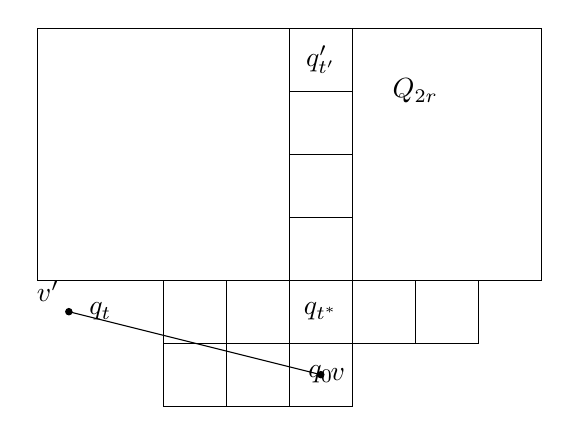
\begin{tikzpicture}[scale=0.8]
    % Define the grid
    \draw[step=1cm] (0,0) grid (3,1);  % Bottom row
    \draw[step=1cm] (0,1) grid (5,2);  % Middle row
    \draw[step=1cm] (2,2) grid (3,6);  % Vertical column
    
    % Draw the L-shaped grid outline
    \draw (0,0) -- (0,2) -- (-2,2) -- (-2,6) -- (6,6) -- (6,2) -- (5,2) -- (5,1) -- (3,1) -- (3,0) -- (0,0);
    
    % Diagonal line from v' to v
    \draw (-1.5,1.5) -- (2.5,0.5);
    
    % Points and labels
    \filldraw (-1.5,1.5) circle (0.05) node[above left] {$v'$};
    \node at (-1,1.5) {$q_t$};
    \node at (2.5,1.5) {$q_{t^*}$};
    \node at (2.5,0.5) {$q_0$};
    \filldraw (2.5,0.5) circle (0.05) node[right] {$v$};
    \node at (2.5,5.5) {$q'_{t'}$};
    
    % Label for Q_{2r}
    \node at (4,5) {$Q_{2r}$};
\end{tikzpicture}

\end{document}